\chapter{Reflexion und Fazit}
\label{chapter:conclusion}

Nachdem in den vorherigen Kapiteln die Durchführung des praktischen
Designprozesses ausführlich beschrieben wurde, soll dieses Kapitel die
Ausarbeitung abschließen, indem es die Ergebnisse zusammenfasst und
hinterfragt. Zunächst wird im Abschnitt \ref{subsection:resultDescription} das
Ergebnis des Gestaltungs- und Entwicklungsprozesses resümiert. Hier wird
nochmals darauf eingegangen, wie der Nutzungskontext erfasst wurde, die
Nutzungsanforderungen spezifiziert, die entsprechenden Gestaltungslösungen
umgesetzt und evaluiert wurden. Somit wird der in den Kapiteln
\ref{chapter:user-context} bis \ref{chapter:evaluation} ausführlich
dokumentierte Entwicklungsprozess nochmals anhand der vier Phasen des Human
Centered Design aufgegriffen und eingeordnet\cite{ISO9241}. Zusätzlich wird
kurz präsentiert, welche Änderungen an der Software nach der Auswertung des
Usertests noch vorgenommen wurden. Als nächstes werden die eingesetzten
Methoden im Abschnitt \ref{subsection:reflection} aufgegriffen und kritisch
hinterfragt. Der Fokus liegt dabei auf der Methode des Interviews im Kontext
und auf dem Designzyklus des Human Centered Design nach ISO9241. Hierbei soll an
die Fragestellung der Einleitung angeknüpft werden und eine Verbindung zu den
gewonnenen Resultaten hergestellt werden. Als Letztes wird in Abschnitt
\ref{subsection:outlook} ein Ausblick gegeben, wie die entwickelte Software nun
in der Praxis eingesetzt werden kann und welche Schritte dazu noch notwendig
sind. Außerdem wird auch skizziert, welche weiteren wissenschaftlichen Methoden
und Prozesse man noch anwenden könnte, um die hier gewonnen Ergebnisse zu
vertiefen und weiter zu verwenden.

\section{Zusammenfassung der Ergebnisse}
\label{subsection:resultDescription}

\subsection*{Was war geplant, was wurde umgesetzt?}
Ziel dieses Abschnittes soll es sein, den Bogen zu spannen zwischen den
anfänglich erarbeiteten Nutzungsanforderungen und den am Ende tatsächlich
umgesetzten Ergebnissen.

Wenn man sich die Auswertung des Interviews im Kontext in Abschnitt
\ref{subsection:IIK} ansieht, wird klar, dass eines der wichtigsten Bedürfnisse
der Nutzenden stets das schnelle und intuitive Nutzen der Software ist. Es
sollten möglichst viele Informationen auf einen Blick sichtbar sein, ohne die
Nutzenden von den wesentlichen Dingen abzulenken. Wenn Workflows durch die
Nutzenden abzuarbeiten sind, sollten diese möglichst schnell und mit möglichst
wenigen Klicks zu erledigen sein. Ein großer Detailgrad der Auswahl- und
Konfigurationsmöglichkeiten sind dagegen in diesem Kontext nicht relevant. Wo
die Software eine halbwegs sinnvolle Vorauswahl treffen kann, sollte dies
automatisch passieren und den Nutzenden somit unnötige Interaktion ersparen.

Um hierfür konkrete Anhaltspunkte zu geben, werden im Folgenden die drei
exemplarisch vorgestellten Nutzungsanforderungen aus Abschnitt
\ref{subsection:SpannendeErkenntnisse} nochmals aufgegriffen.

Gefordert wurde da eine kompakte Kalenderansicht, die durch farbliche
Markierungen auf den ersten Blick darstellt, an welchen Tagen noch freie
Termine verfügbar sind. Diese Anforderung konnte durch die tabellarische
Monatsansicht mithilfe der Javascript Bibliothek \textit{fullcalendar}
umgesetzt werden. Durch die roten und grünen Punkte neben jedem angezeigten
Termin kann direkt auf den ersten Blick erkannt werden, ob es sich um einen
bereits vergebenen oder freien Termin handelt. Durch die verwendete Bibliothek
zum Darstellen der Monatsübersicht ist dieser tabellarische Überblick nicht
mehr ganz so kompakt wie in der alten Softwareversion. Dies ist auch \ipName
beim Usertest negativ aufgefallen. Ein positiver Ausgleich hierfür ist
allerdings, das in der neuen Übersicht direkt die einzelnen Termine eines Tages
dargestellt werden. In der alten Version war es nötig, zunächst den Tag
anzuklicken und erst in dem danach erscheinenden Modal konnten die einzelnen
Termine und die entsprechenden Uhrzeiten eigensehen werden. Der etwas
ausführlichere neue View nimmt also mehr Platz auf dem Bildschirm ein und kann
bei sehr vielen Terminen an einzelnen Tagen sehr lang werden, bietet dafür aber
eine umfassende Übersicht über freie und vergebene Termine und stellt
weiterführende Informationen mit nur einem Klick in der Detailansicht zur
Verfügung.

\begin{figure}[H]
    \caption{Vergleich der Monatsübersicht in der alten und neuen Softwareversion.}
    \centering
    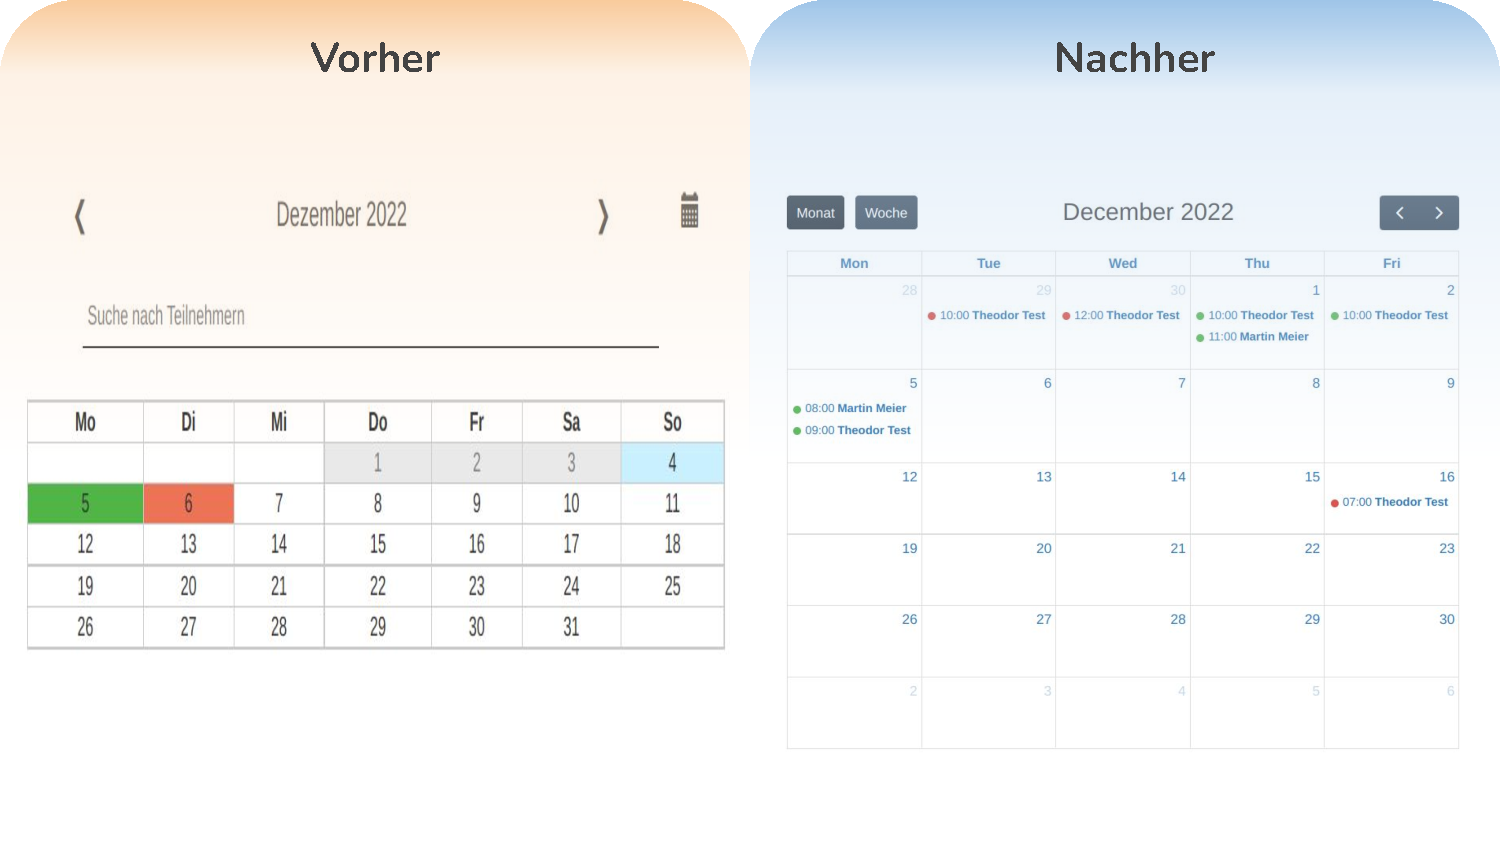
\includegraphics[width=\textwidth]{screen_past_now_month_view.pdf}
\end{figure}

Als nächstes wurde beim Interview im Kontext deutlich, dass eine Funktion
notwendig ist, um im Nachhinein den Termin eines Ratsuchenden schnell und
unkompliziert finden zu können. Hierfür wurde die Suchfunktion neu
implementiert. Bereits nach dem Eingeben einiger Buchstaben aus dem Namen der
ratsuchenden Person schlägt diese neue Suchfunktion passende Ergebnisse vor und
bietet in einer tabellarischen Übersicht direkt die wichtigsten Daten zum
zugehörigen Beratungstermin. Durch einen Klick auf ein Suchergebnis kann der
Termin schnell und einfach in der Detailansicht geöffnet werden. In der
Planungsphase war hierfür ein extra Button mit einem Augensymbol vorgesehen.
Ein einfacher Klick auf die entsprechende Zeile in der Tabelle hat sich aber
als praktischer erwiesen. Im Vergleich zur alten Softwareversion sind die
Suchergebnisse sehr viel ausführlicher und strukturierter dargestellt. Dies
wurde auch im Usertest positiv wahrgenommen. In weiteren Tests entsteht der
Eindruck, dass die alte Suchfunktion etwas schneller gearbeitet hat. Dies kann
aber erst objektiv bewertet werden, wenn die neue Implementierung auch auf den
gleichen Produktiv-Servern installiert und im Einsatz ist.

\begin{figure}[H]
    \caption{Vergleich der Suchfunktion in der alten und neuen Softwareversion.}
    \centering
    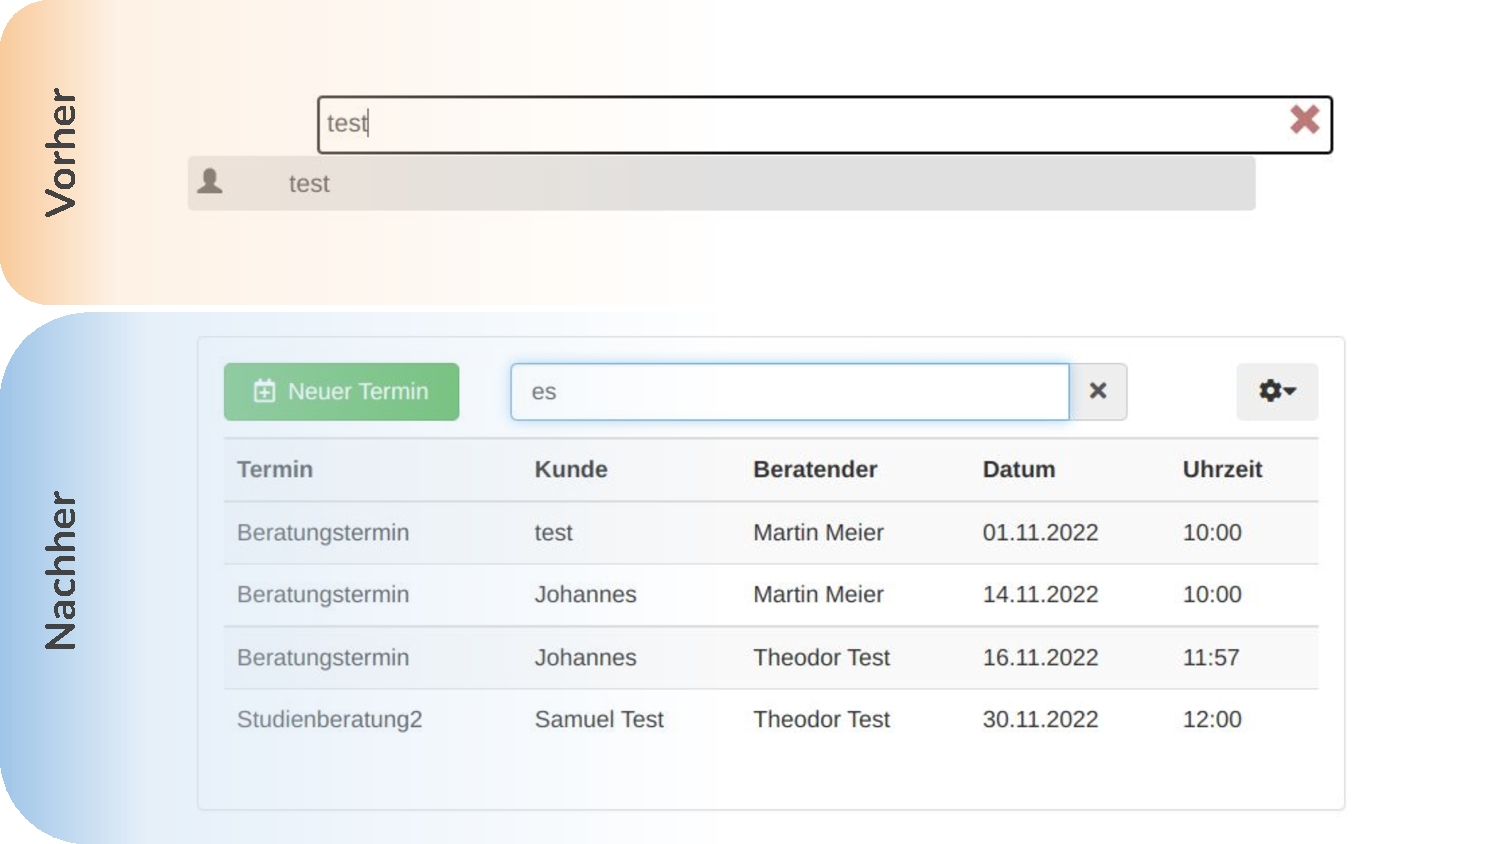
\includegraphics[width=\textwidth]{screen_past_now_search.pdf}
\end{figure}

Als letztes wurde im Abschnitt \ref{subsection:SpannendeErkenntnisse} das
elegante Darstellen der Telefonnummern gefordert. Dieses Feature ließ sich in
der Praxis leicht implementieren. In die aus der Datenbank abgerufene 
Telefonnummer wird an jeder vierten Stelle ein Leerzeichen eingefügt. Somit
kann die Telefonnummer von den Studienberatenden bei Bedarf in leicht zu
merkenden Vierer-Blöcken in das Telefon eingeben werden. Für andere
Nutzeraccounts als den zuständigen Beratenden werden persönliche Details der
Ratsuchenden nicht angezeigt. Diese Funktion gab es bereits in der alten Version, allerdings wird in der neuen Version statt den eigentlichen Daten ein
Hinweis angezeigt. In der alten Version wurde an dieser Stelle gar nichts
angezeigt, was manchmal zu Unsicherheiten geführt hat, ob hier überhaupt Daten
eingetragen und korrekt gespeichert wurden. Das Feedback aus dem Usertest
zeigt: Die neue Variante braucht etwas mehr Platz auf dem Bildschirm, ist dafür
aber klarer zu verstehen und intuitiver zu erfassen.

\begin{figure}[H]
    \caption{Vergleich der Detailansicht eines vergebenen Termins in der alten und neuen Softwareversion.}
    \centering
    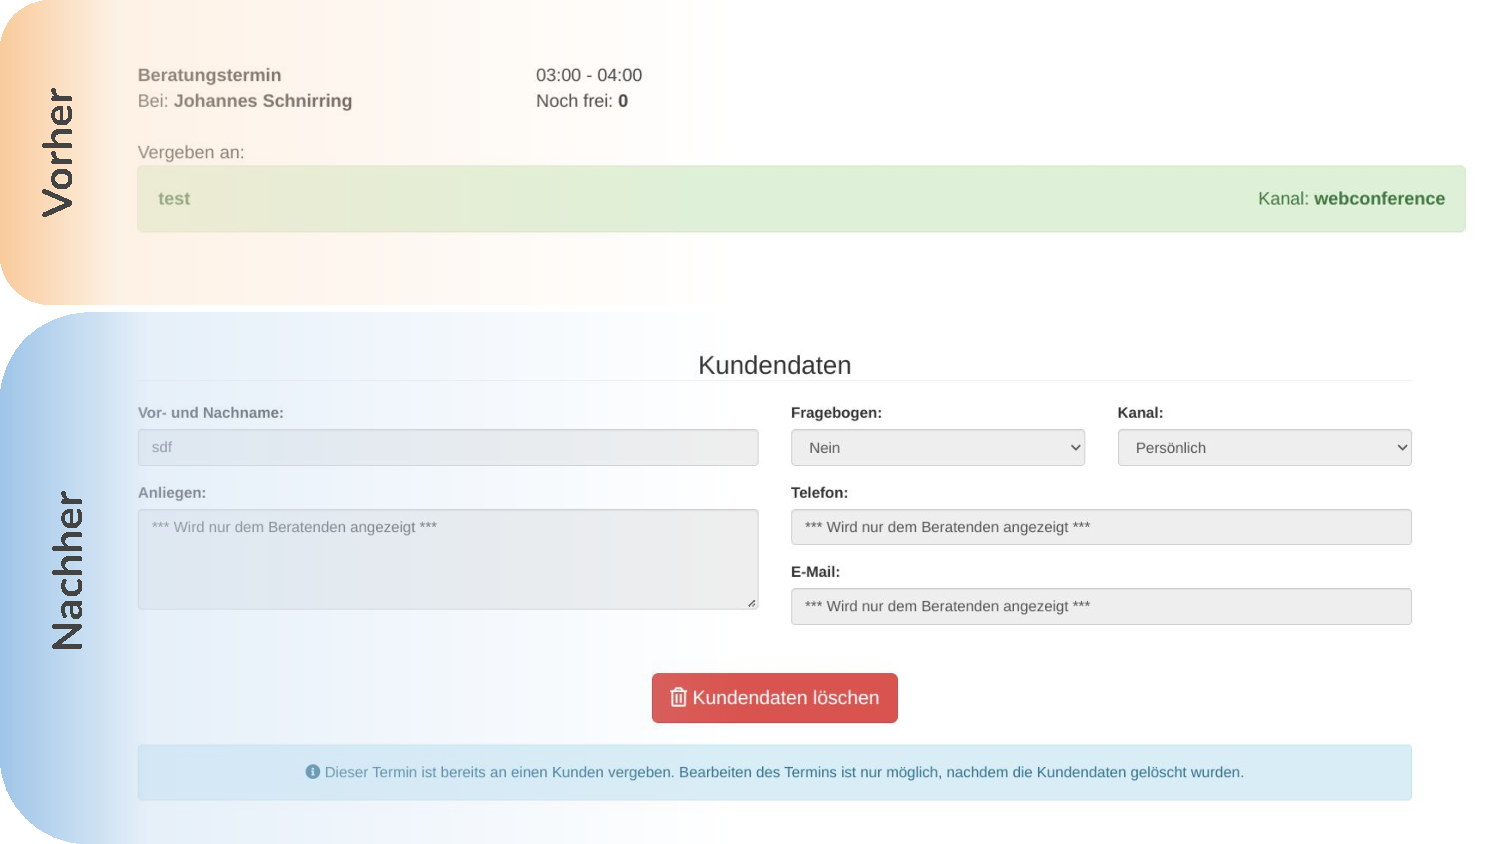
\includegraphics[width=\textwidth]{screen_past_now_client_details.pdf}
\end{figure}

\subsection*{Umsetzung von Feedback des Usertests}
\label{paragraph:weitereIteration}

In den Kapiteln \ref{chapter:user-context} bis \ref{chapter:evaluation} wurde
das Durchlaufen des Designzyklus anhand einer Iteration ausführlich
beschrieben. Ein essentielles Grundkonzept des Human Centered Design beinhaltet
allerdings auch das Durchlaufen weiterer Iterationen\cite{hcd}. K. Holtzblatt
betont in \textit{Contextual Design: Evolved}, dass der Entwicklungsprozess mit
einem durchgeführten Usertest noch nicht als abgeschlossen gelten sollte. Die
herausgearbeiteten Kritikpunkte und Verbesserungsvorschläge, die sich aus dem
Usertest ergeben haben, sollten auch in den Gestaltungsprozess der Software mit
einfließen\cite{holtzblattCDEvolved}. Dies ist im Schaubild nach ISO9241 durch
die gestrichelten Pfeile erkennbar. Nach der Evaluierung sollte der Prozess
erneut durchlaufen werden. Der Einstieg erfolgt dabei je nach Feedback der
Nutzenden in Phase eins bis drei\cite{ISO9241}. Diese weiteren Iterationen
ausführlich zu beschreiben würde den Rahmen dieser Arbeit überstrapazieren.
Daher werden im Folgenden lediglich die Ergebnisse eines zweiten Durchlaufes
nach dem Usertest exemplarisch präsentiert:

Ein neuer Button \textit{Speichern und Nächster} wird beim Erstellen eines
neuen Termins angezeigt. Somit kann mit einem Klick der aktuelle Termin
gespeichert werden und direkt ein neuer Datensatz eingetragen werden. Die
Besonderheit ist, dass die Formularfelder in diesem Fall nicht auf
Standardwerte zurückgesetzt werden. Somit können viele Termine mit ähnlichen
Attributen besonders schnell hintereinander eingetragen werden.

\begin{figure}[H]
    \caption{Neuer Button: Mit \textit{Speichern und Nächster} kann direkt der nächste Termin eingetragen werden.}
    \centering
    
\includegraphics[width=0.9\textwidth]{screen_feedback_save_next.png}
\end{figure}

\ipName hat während des Usertests angemerkt, dass nicht nur das Beratungsanliegen der ratsuchenden Personen besonderem Datenschutz unterliegt. Auch persönliche Kontaktdaten wie Mailadresse und Telefonnummer sollten nur dem zuständigen Beratenden angezeigt werden. In der überarbeiteten Version werden somit nun auch die Telefonnummer und die Mailadresse des Kunden zensiert.

\begin{figure}[H]
    \caption{Details eines vergebenen Termins aus Ansicht einer Hilfskraft.}
    \centering
    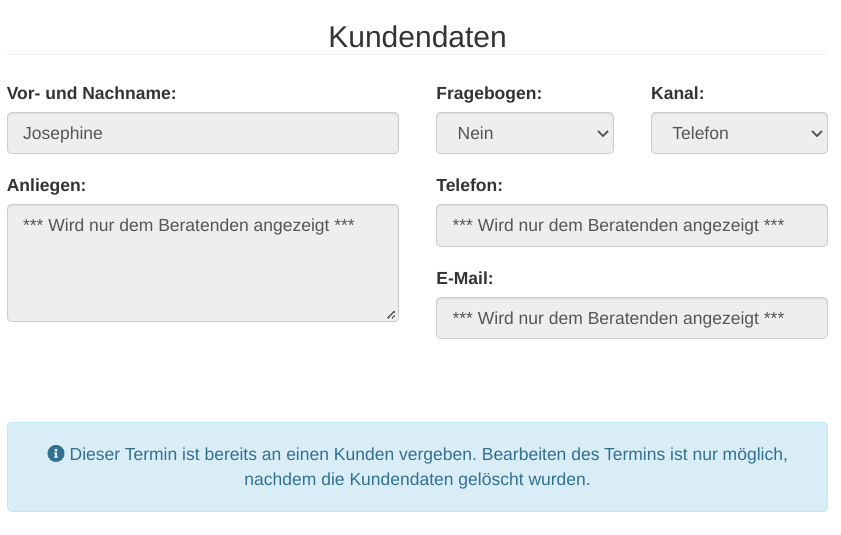
\includegraphics[width=0.9\textwidth]{screen_feedback_client_censorship.png}
\end{figure}

\section{Reflexion der eingesetzen Methoden}
\label{subsection:reflection}

Um dem wissenschaftlichen Anspruch dieser Arbeit Genüge zu tragen, sollen die
vorgestellten Methoden und Theorien nicht nur in der Praxis erprobt, sondern
auch kritisch hinterfragt und eingeordnet werden. Im folgenden Abschnitt werden
die Methoden des Human Centered Design und des Interviews im Kontext nochmals
aufgegriffen und deren Praxistauglichkeit reflektiert. Des Weiteren wird auch
die Umsetzung und Implementierung der Gestaltungslösungen in Frage gestellt und
unter Einbeziehung des Feedbacks aus dem Usertest analysiert.

\subsection*{Human Centered Design und Interview im Kontext}
Die Theorie des Human Centered Design wurde zu Beginn dieser Arbeit motiviert
mit der technischen Entwicklung von interaktiven Systemen. Software ist im
Laufe der letzten Jahrzehnte immer interaktiver geworden. Der Schnittstelle
zwischen Mensch und Maschine kommt dabei eine immer größer werdenden Bedeutung
zu\cite{hci}. Der Ansatz des Human Centered Design versucht an dieser Stelle
alle Beteiligten einzubeziehen und eine einfache, intuitive Bedienung der
Systeme zu ermöglichen, die ganz bewusst aus Perspektive der Nutzenden
gestaltet wurde\cite{sequenceDiagrams}. Diese Theorie wurde in diesem Fall
anhand des Designzyklus nach ISO9241 in die Praxis umgesetzt. Für die
Durchführung der ersten Phase \textit{Den Nutzungskontext verstehen und
    Beschreiben} wurde hier die Methode des Interviews im Kontext verwendet.
Hierbei ging es darum, alle Menschen, die mit dem System zu tun haben
einzubeziehen und ihre Arbeitsabläufe zu verstehen. Wie der Name der Methode
bereits impliziert, liegt der Fokus hierbei auch auf dem Kontext, in dem diese
Arbeitsabläufe stattfinden\cite{hciHandbook}. Das Interview im Kontext wurde
deshalb mit \ipName in seinem Büro an seinem Dienstrechner durchgeführt, um eine
möglichst realistische Alltagssituation abzubilden.

Eine zentrale Fragestellung dieser Arbeit war folgendermaßen beschrieben
worden: \textit{An welchen Stellen können die theoretischen Grundlagen des
    Human Centered Design den Entwicklungsprozess in der Praxis tatsächlich
    sinnvoll unterstützen?} Der Einsatz dieser Methoden lässt sich rückblickend als
sehr ertragreich beschreiben. Durch den engen Austausch mit \ipName konnte der
Nutzungskontext sehr gut verstanden und aufgearbeitet werden. Das Interview im
Kontext hat überraschend viele neue Ideen hervorgebracht, die wohl keiner der
Beteiligten im Vorhinein hätte formulieren können. Durch das gemeinsame
Benutzen der alten Softwareversion vor Ort wurde ganz klar deutlich, welche
Features wirklich wichtig sind für den täglichen Einsatz, an welchen Stellen es
schnell gehen muss und wo detaillierte Einstellungsmöglichkeiten unbedingt
notwendig sind. Die Erkenntnisse und Beobachtungen aus dem Interview im Kontext
wurden unstrukturiert schriftlich festgehalten. Beim Auswerten dieser Notizen
ist aufgefallen, dass viele Details aus dem Gespräch nicht so schnell
aufgeschrieben werden konnten. Die Notizen waren somit nicht ganz vollständig.
Daher war es sehr wichtig, die Auswertung des Interviews im Kontext zeitlich
sehr nah an der Durchführung zu planen. Somit konnten viele Details aus der
Erinnerung an das Interview selbst bei der Auswertung ergänzt werden. Der
Austausch mit Menschen aus der allgemeinen Studienberatung hat sich auf den Kontakt
mit \ipName beschränkt. Dieser Austausch war sehr ertragreich, dennoch wäre es
interessant gewesen, auch noch Nutzungsanforderungen anderer Nutzergruppen wie
beispielsweise der Hilfskräfte der Erstinformation mit einzubeziehen. Die
Erfahrungen und Ideen anderer Nutzenden hätten noch weitere hilfreiche Aspekte
in den Gestaltungsprozess einbringen können. Somit hätte ein System entstehen
können, das noch inklusiver und reibungsloser alle beteiligten Personen mit
einbezieht. In der Praxis war es allerdings schon sehr aufwendig, Termine mit
\ipName zu organisieren. Wären noch weitere Nutzungsgruppen mit einbezogen
worden, wäre der organisatorische und zeitliche Aufwand der Software deutlich
höher gewesen. Dies kann gerade in gewinnorientierten Softwarehäusern einen
hemmenden Faktor für den Einsatz von Human Centered Design mit sich bringen.

Um noch einmal Bezug auf die vier Phasen des Gestaltungsprozesses nach ISO9241
zu nehmen, kann man festhalten, dass die klare Zuordnung der Arbeitsschritte in
eine dieser Phasen sehr gut funktioniert hat. Somit wurde jede Arbeitsphase
klar strukturiert und war einem definierten Ergebnis zugeordnet. Ein
zielführendes und effizientes Arbeiten wurde somit erleichtert.

\subsection*{Implementierung und Usertests}

Im Folgenden soll nun auch die Implementierung der Software kritisch
hinterfragt werden. Die Ergebnisse der Usertests sollen hierbei mit einbezogen
werden und das Meinungsbild mit ersten Testerfahrungen bestärken.

% Einfache Umsetzung vs Nutzerfreundliche Lösung
Zunächst fällt allgemein auf, dass besonders nutzungsfreundliche Lösungen
oftmals technisch verhältnismäßig aufwendig umzusetzen sind. Wird Software von
Seite der technischen Möglichkeiten und Datenstrukturen her gestaltet, drängen
sich bestimme Herangehensweisen oftmals fast unumgänglich auf. Diese
Herangehensweisen sind dann meist sehr technisch geprägt und für unerfahrene
Nutzende manchmal schwierig zu verstehen. Wenn man diesen Prozess im Sinne des
Human Centered Design bewusst umdreht und die Gestaltung bei den Nutzenden und
ihrem Umfeld beginnt, können oftmals deutlich passendere und einfachere
Workflows und Views geschaffen werden. Diese sind in der Implementierung
allerdings oftmals aufwendig zu realisieren.

% Problem: Designpattern bei fertigem Softwareökosystem sehr eingeschränkt
% Objektorientierter Ansatz sinnvoll für start serverlastige Anwendung?
Als nächstes soll nochmal in Erinnerung gerufen werden, dass es sich bei dieser
Umsetzung um ein Modul in einer bereits bestehenden Software handelt. Es
mussten also alle bestehenden Schnittstellen und Programmierkonzepte der
bereits existierenden Module eingehalten werden. Beispielsweise wurde für die
Termindatensätze, sowie für Beratungsräume und Mailtemplates, ein
objektorientierter Ansatz gewählt. Ziel war es, damit die Beziehungen dieser
Datentypen untereinander klarer modellieren und elegant in Code umsetzen zu
können. Im Rahmen der gesamten Software Stubegru hat sich allerdings gezeigt,
das es eher wenig Sinn macht, lokale Instanzen von Objekten zu erstellen und zu
referenzieren. Die restlichen Module funktionieren so, dass Daten meist nur vom
Server abgerufen und angezeigt werden. Weitere Referenzen oder Methodenaufrufe
auf diesen Daten sind nicht vorgesehen und machen in diesem Anwendungsfall auch
wenig Sinn. Die erhofften Vorteile der objektorientierten Umsetzung in diesem
Modul konnten somit nicht vollständig erreicht werden. Viele Methoden wurden
letztendlich als \textit{static} implementiert und werden somit unabhängig von
der Instanz einer Klasse aufgerufen.

% Prototypen wichtig für Feedback, Vorstellung
% Evtl frühere Tests
Im Usertest hat sich herausgestellt, dass es extrem hilfreich ist, wenn man
eine Gestaltungslösung vorzeigen und gemeinsam durchspielen kann. Beim
gemeinsamen Nutzen der implementierten Funktionen fallen oft wichtige Details
auf, die im Vorhinein bei der Planung noch nicht berücksichtigt wurden. Somit
war es also extrem hilfreich, für den Usertest bereits das fast vollständig
fertig implementierte Modul zur Terminvereinbarung präsentieren zu können und
somit eine greifbare Gesprächsgrundlage zu bieten. Vielleicht wäre es hilfreich
gewesen, schon früher im Gestaltungsprozess erste Prototypen zu entwickeln, die
noch nicht voll funktionstüchtig sind, allerdings schon die wichtigsten
Nutzungsinteraktionen wiedergeben können. Dann hätte man den Nutzenden schon
früher im Designprozess ein anschauliches Beispiel für konkrete
Gestaltungslösungen präsentieren können. Somit hätten etwaige Mängel schon
früher erkannt und direkt korrigiert werden können. Allerdings lässt sich
auch festhalten, dass durch das ausführliche Interview im Kontext bereits ein
sehr guter Überblick entstanden ist, wie die Software aussehen sollte, um die
Nutzenden möglichst gut zu unterstützen. Somit waren nach dem Usertest gar
keine großen, grundlegenden Änderungen mehr notwendig. Dies zeigt auf, dass
eine ausführliche und gewissenhafte Durchführung der ersten Phasen im
Gestaltungsprozess die Wahrscheinlichkeit für Missverständnisse oder größere
Änderungswünsche in späteren Usertests senkt.

\section{Ausblick}
\label{subsection:outlook}

Als abschließender Abschnitt dieser Ausarbeitung soll die weitere Perspektive
des Forschungsthemas betrachtet werden. Hierbei ist es interessant, den weiteren
Einsatz des praktisch entwickelten Moduls zur Terminvereinbarung zu skizzieren.
Wie wird sich das Modul in das gesamte Softwarepaket Stubegru eingliedern? In
welchem Kontext kann es tatsächlich produktiven Einsatz finden und welche
Schritte sind dafür noch zu bedenken? Außerdem sollen die verwendeten Methoden
und Theorien nochmals aufgegriffen werden. An welchen Stellen lassen sich die
verwendeten Konzepte eventuell noch verbessern? In welcher Richtung verspricht
eine weitere wissenschaftliche Forschung spannende neue Erkenntnisse?

\subsection*{Werdegang der Software Stubegru}
Wie bereits in Abschnitt \ref{paragraph:weitereIteration} erwähnt, sind noch
weitere Iterationen und Feedbackrunden mit den Nutzenden nötig, um das neu
entwickelte Modul zur Terminvereinbarung tatsächlich sinnvoll im Arbeitsalltag
zu verwenden. Es ist konkret geplant, diese weiteren Entwicklungszyklen zu
durchlaufen und eine neue Version der Software Stubegru in der Abteilung
Studium und Lehre produktiv einzusetzen. Ist das Modul zur Terminvereinbarung
fertig, werden noch andere Module und Workflows der Software überarbeitet
werden müssen. Wenn all diese Arbeiten abgeschlossen sind, wird es eine
intensive Einführungsphase geben. In den ersten Wochen im produktiven Betrieb
ist zu erwarten, dass noch einige Bugs entdeckt und behoben werden müssen.
Außerdem müssen die Mitarbeitenden der Abteilung auf die neuen Abläufe in der
überarbeiteten Softwareversion geschult werden. All diese Schritte sollen im
Rahmen eines Dienstleistungsvertrages mit der Universität Kassel weiterhin
betreut werden.

\subsection*{Forschungsausblick}
Die Durchführung und Auswertung dieser Arbeit hat gezeigt, dass die verwendeten
Theorien des Human Centered Design schon sehr ausgereift und vor allem sehr
praxisnah formuliert sind. Die Umsetzung der methodischen Grundkonzepte ließ
sich somit sehr gut in die Praxis übertragen. Spannend wäre es allerdings, sich
noch tiefgreifender mit den verschiedenen Nutzungsgruppen einer Software
auseinander zu setzen. In dieser Arbeit bedeutete der Austausch mit den
Nutzenden größtenteils der Kontakt mit einem Studienberater der allgemeinen
Studienberatung. Dieser repräsentierte eine Nutzungsgruppe, die bereits
jahrelange Erfahrung mit den Prozessen und Abläufen in der Abteilung vorweisen
kann. Spannend wäre es, noch weitere Nutzungsgruppen in den Fokus zu rücken.
Hilfskräfte beispielsweise sind oftmals nur für einen kurzen Zeitraum mit
geringen Wochenstunden angestellt. Eine jahrelange Einarbeitung in die Prozesse
des Arbeitsalltags kann hier nicht vorausgesetzt werden. Wie könnte man also
diese Nutzungsgruppe besser in der Bedienung der verwendeten Software
unterstützen? Könnten zum Beispiel kleine interaktive Hilfetexte helfen, die
Arbeitsprozesse spielerisch bei der Verwendung der Software zu erlernen?
Hierfür wäre sicherlich ein intensiverer und direkter Austausch mit
Hilfskräften der Abteilung notwendig gewesen.

Des Weiteren wäre es relevant, die Unterschiede in der direkten Interaktion mit
dem Computer der einzelnen Nutzenden genauer zu untersuchen. In den hier
verwendeten Grundlagen zum Human Centered Design lag der Fokus immer darauf,
eine Gestaltungslösung zu finden, die möglichst nutzungsfreundliche
Schnittstellen bietet\cite{hcd}. Oftmals bevorzugen verschiedene Nutzende
allerdings verschiedene Schnittstellen. Ich persönlich, als technisch sehr
erfahrener Nutzer, bevorzuge beispielsweise Eingaben über die Tastatur und
arbeite gerne mit Shortcuts. In den Usertests hat sich schnell gezeigt, dass
der Testkandidat am liebsten alle Formularfelder mit der Maus ausfüllt. Somit
ist für ihn beispielsweise ein grafischer Timepicker sehr wichtig für eine gute
User Experience. Für mich wäre es allerdings viel wichtiger, die Möglichkeit zu
haben, jedes Eingabefeld auch über Tastaturbefehle zu erreichen. Dieses kleine
Beispiel soll illustrieren, dass selbst einzelne Menschen einer Nutzungsgruppe
oftmals ganz verschiedene Vorstellungen von einer \textit{angenehmen} und
\textit{schönen} Nutzungsoberfläche haben. Diese Differenzen weiter zu
untersuchen und allen Nutzenden eine adäquate Schnittstelle zu bieten, wäre also
eine weitere spannende Richtung, um die Ergebnisse dieser Arbeit noch weiter zu
vertiefen.